\chapter{Random Forest}
\label{chap:randomforest}

\begin{myremark}[Algorithmusart in diesem Kapitel]
Funktionsart: \textbf{Klassifikation}. \\
Umsetzungsart: \textbf{datengetrieben} (Ensembleverfahren).
\end{myremark}

\begin{myremark}
Der \textbf{Random Forest} baut auf dem Entscheidungsbaum auf (Kapitel~\cref{chap:entscheidungsbaum}) und macht ihn
durch \enquote{Ensembling} deutlich robuster. Diese Methode setzt Kenntnisse aus Kapitel~\cref{chap:entscheidungsbaum} voraus.
\end{myremark}

\section{Grundidee: Viele Bäume, eine Entscheidung}

\begin{mydefinition}[Random Forest]
Ein \textbf{Random Forest} kombiniert viele \textbf{zufällig variierte} Entscheidungsbäume.
Die finale Klassifikation entsteht durch \textbf{Mehrheitsabstimmung} aller Bäume.
\end{mydefinition}

Durch zwei Mechanismen wird jeder Baum bewusst \enquote{anders} gemacht:
\begin{enumerate}
    \item \textbf{Bagging:} Jeder Baum trainiert auf einer zufälligen Stichprobe der Daten
          (mit Zurücklegen).
    \item \textbf{Feature-Subsampling:} An jedem Knoten wird nur eine zufällige Teilmenge
          der Merkmale betrachtet.
\end{enumerate}

\begin{figure}[H]
    \centering
    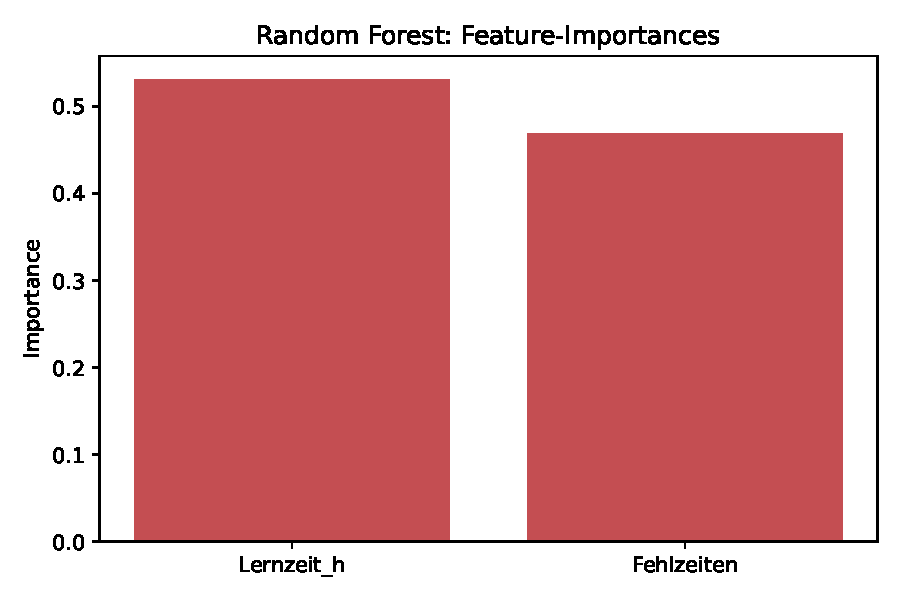
\includegraphics[width=0.72\textwidth]{Grundlagen_Info/15_KI_und_Algorithmen/Figures/random_forest_feature_importance.pdf}
    \caption{Feature-Importances eines Random-Forest-Modells}
    \label{fig:rf-importance-15}
\end{figure}

\section{Feature Importance}

\begin{mydefinition}[Feature Importance]
Der Random Forest kann angeben, wie stark jedes Merkmal zur Entscheidung beiträgt.
Ein Merkmal ist wichtig, wenn Splits auf ihm die Unreinheit (Gini) stark reduzieren.
\end{mydefinition}

\begin{myexercise}[Vergleich: Baum vs.\ Wald]
Diskutieren Sie in Zweiergruppen:
\begin{itemize}
    \item Warum kann ein einzelner Baum schnell \enquote{auswendig lernen}?
    \item Warum ist ein Wald oft robuster gegen Overfitting?
    \item Welche Nachteile hat der Random Forest gegenüber einem einzelnen Baum?
\end{itemize}
\end{myexercise}

\section{Hyperparameter}

\begin{mychallenge}[Hyperparameter verstehen und tunen]
Recherchieren und erklären Sie kurz:
\begin{itemize}
    \item \texttt{n\_estimators} – Anzahl Bäume
    \item \texttt{max\_depth} – maximale Tiefe je Baum
    \item \texttt{min\_samples\_leaf} – Mindestgrösse eines Blatts
\end{itemize}
Testen Sie im Notebook verschiedene Werte und dokumentieren Sie den Effekt
auf Trainings- und Testgenauigkeit.
\end{mychallenge}

\begin{myremark}[Notebook]
Praktische Umsetzung inkl. Übungen:
\href{\notebookbaseurl02_Random_Forest_Classification.ipynb}{\texttt{02\_Random\_Forest.ipynb}}
\end{myremark}
